%\title{DeToanMinhHoa2017-Đề nghị không sửa đổi}
\documentclass[12pt]{examdesign}
\usepackage{fourier}
\usepackage{amsmath,amsxtra,latexsym, amssymb, amscd}
\usepackage[mathletters]{ucs}
\usepackage[utf8x]{inputenc}
\usepackage[utf8]{vietnam}
\usepackage{color}
\usepackage{graphicx}
\usepackage{wrapfig}
\usepackage{times}
\usepackage{dethi} 
\usepackage[a4paper,tmargin=1.0cm, bmargin=1.5cm, lmargin=1.5cm, rmargin=1.5cm]{geometry}
\ContinuousNumbering 
\ShortKey
\NumberOfVersions{1} % số bài thi khác nhau được in ra
\SectionPrefix{\relax }
% Tiêu đề 
\tentruong{SỞ GIÁO DỤC VÀ ĐÀO TẠO BÌNH DƯƠNG}
\loaidethi{ĐỀ THI MẪU} % ĐỀ THI CHÍNH THỨC 
\Sotrang{Đề thi gồm có 5 trang}  % nếu sửa ở đây thì sửa luôn ở dòng 35
\tenkythi{KỲ THI THỬ THPT QUỐC GIA NĂM 2017}
\tenmonhoc{Môn: Toán}
\madethi{100}\bigskip

\thoigian{\underline{Thời gian làm bài: 90 phút, không kể thời gian phát đề}}

% hết tiêu đề 

\tieudetracnghiem
\tieudedapan
\tieudeduoi
\daungoac{}{.}
\chucauhoi{Câu} 
\mauchu{black}
\sotrang{5}
\renewcommand{\baselinestretch}{1.125}
\NoRearrange

\newcommand{\chenhinhve}[3]{
\begin{wrapfigure}{r}{#1}\examvspace*{#3}\includegraphics[width=#1]{#2}\end{wrapfigure}
}


\begin{document}

%\begin{vnmultiplechoice}[ rearrange=no, keycolumns=5]%
\begin{vnmultiplechoice}[ rearrange=yes, keycolumns=5]%

\begin{question}%1
Đường cong trong hình bên là đồ thị của một hàm số trong bốn hàm số 

\chenhinhve{4cm}{toan01}{-1.5cm}
được liệt kê ở bốn phương án $A, B, C, D$ dưới
đây.
 Hỏi hàm số đó là hàm số nào?
\datcot
\bonpa
{\sai{$y=-x^2+x-1$.}}
{\sai{$y=-x^3+3x+1$.}}
{\dung{$y=x^3-3x+1$.}}
{\sai {$y=x^4-x^2+1$.}}
\end{question}


\begin{question}%2
Cho hàm số $y=f(x)$ có  $\lim\limits_{x\rightarrow +\infty}=1$ và   $\lim\limits_{x\rightarrow -\infty}=-1$. Khẳng định nào sau
đây là khẳng định đúng ?
\datcot[4]
\bonpa
{\sai{Đồ thị hàm số đã cho không có tiệm cận ngang.}}
{\sai{Đồ thị hàm số đã cho có đúng một tiệm cận ngang.}}
{\dung{Đồ thị hàm số đã cho có hai tiệm cận ngang là các đường thẳng  $y=1$ và  $y=-1$.}}
{\sai {Đồ thị hàm số đã cho có hai tiệm cận ngang là các đường thẳng $x=1$ và  $x=-1$.}}
\end{question}


\begin{question}%3
 Hỏi hàm số $y=2x^4+1$  đồng biến trên khoảng nào ?
\datcot[2]
\bonpa
{\sai{$\left(-\infty; -\frac{1}{2}\right)$.}}
{\dung{$\left(0;+\infty\right)$.}}
{\sai{$\left(-\frac{1}{2}; +\infty\right)$.}}
{\sai {$(-\infty;0)$.}}
\end{question}

\begin{question}%4
Cho hàm số  $y=f(x)$ xác định, liên tục trên $\mathbb{R}$ và có bảng biến thiên:

\begin{wrapfigure}[10]{r}[-5cm]{2cm}
\examvspace*{-0.5cm}
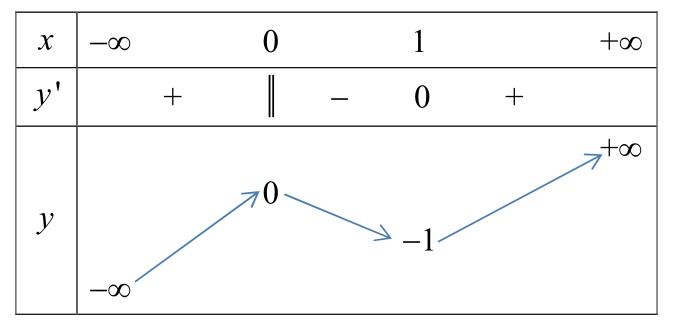
\includegraphics[scale =0.5]{toan02}
\end{wrapfigure}
Khẳng định nào sau đây là khẳng định đúng ?
\datcot[4]
\bonpa
{\sai{Hàm số có đúng một cực trị.}}
{\sai{Hàm số có giá trị cực tiểu bằng $1$.}}
{\sai {Hàm số có giá trị lớn nhất bằng $0$ và giá trị nhỏ nhất bằng  $1$.}}
{\dung{Hàm số đạt cực đại tại  $x=0$ và đạt cực tiểu tại  $x=1$.}}
\end{question}


\begin{question}%5
Tìm giá trị cực đại $y_{\mbox{\scriptsize  \textit{CĐ} }}$ của hàm số $y=x^3-3x+2$.
\datcot
\bonpa
{\dung{$y_{\mbox{\scriptsize \textit{CĐ} }}=4$.}}
{\sai{$y_{\mbox{\scriptsize \textit{CĐ} }}=1$.}}
{\sai{$y_{\mbox{\scriptsize  \textit{CĐ} }}=0$.}}
{\sai {$y_{\mbox{\scriptsize \textit{CĐ} }}=-1$.}}
\end{question}


\begin{question}%6
Tìm giá trị nhỏ nhất của hàm số $y=\dfrac{x^2+3}{x-1}$ trên đoạn $[2;4]$.
\datcot
\bonpa
{\dung{$\underset{[2;4]} \min y=6$..}}
{\sai{$\underset{[2;4]} \min y=-2$.}}
{\sai{$\underset{[2;4]} \min y=-3$.}}
{\sai {$\underset{[2;4]} \min y=\dfrac{19}{3}$.}}
\end{question}

\begin{question}%7
Biết rằng đường thẳng  $y=-2x+2$ cắt đồ thị hàm số
$y=x^3+x+2$ tại điểm
duy nhất; kí hiệu
$(x_0;y_0)$ là tọa độ của điểm đó. Tìm $y_0$.
\datcot
\bonpa
{\sai{$y_0=4$.}}
{\sai{$y_0=0$.}}
{\dung{$y_0=2$.}}
{\sai {$y_0=-1$.}}
\end{question}

\begin{question}%8
Tìm tất cả các giá trị thực của tham số $m$ sao cho đồ thị của hàm số $y=x^4+2mx^2+1$ có ba điểm cực trị tạo thành một tam giác vuông cân.
\datcot
\bonpa
{\sai{$m=-\dfrac{1}{\sqrt[3]{9}}$.}}
{\dung{$m=-1$.}}
{\sai{$m=\dfrac{1}{\sqrt[3]{9}}$.}}
{\sai {$m=1$.}}
\end{question}


\begin{question}%9
Tìm tất cả các giá trị thực của tham số $m$ sao cho đồ thị của hàm số $y=\dfrac{x+1}{\sqrt{m x^2+1}}$
\datcot[4]
\bonpa
{\sai{Không có giá trị thực nào của m thỏa mãn yêu cầu đề bài.}}
{\sai{$m<0$.}}
{\sai {$m=0$.}}
{\dung{$m>0$.}}
\end{question}

\begin{question}%10
Cho một tấm nhôm hình vuông cạnh 12 cm.

\begin{wrapfigure}[10]{r}[-6.5cm]{2cm}
\examvspace*{-1.cm}
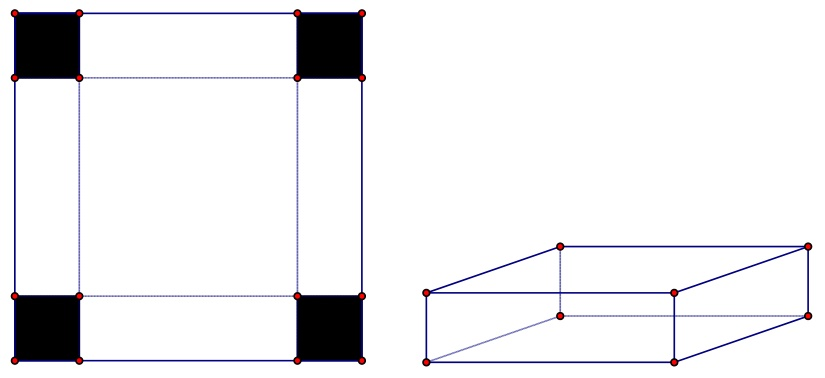
\includegraphics[scale =0.5]{toan03}
\end{wrapfigure}
Người ta cắt ở bốn góc của tấm
nhôm đó bốn hình vuông bằng nhau, mỗi hình vuông có cạnh bằng $x$ (cm), rồi gập tấm
nhôm lại như hình vẽ dưới đây để được một cái hộp không nắp. Tìm $x$ để hộp nhận
được có thể tích lớn nhất.
\datcot
\bonpa
{\sai{$x=6$.}}
{\dung{$x=3$.}}
{\sai{$x=2$.}}
{\sai {$x=4$.}}
\end{question}

\begin{question}%11
Tìm tất cả các giá trị thực của tham số $m$ sao cho hàm số $y=\dfrac{\tan x-2}{\tan x -m}$ đồng biến trên $\left(0;\dfrac{\pi}{4}\right)$.
\datcot[2]
\bonpa
{\dung{$m\le 0$ hoặc $1\le m <2$.}}
{\sai{$m\le 0$.}}
{\sai{$\le m < 2$.}}
{\sai {$m\ge 2$.}}
\end{question}

\begin{question}%12
Giải phương trình $\log_4(x-1)=3$.
\datcot
\bonpa
{\sai{$x=63$.}}
{\dung{$x=65$.}}
{\sai{$x=80$.}}
{\sai {$x=82$.}}
\end{question}


\begin{question}%13
Tính đạo hàm của hàm số $y=13^x$.
\datcot
\bonpa
{\sai{$y'=x.13^{x-1}$.}}
{\dung{$y'=13^{x}.\ln 13$.}}
{\sai{$y'=13^{x}$.}}
{\sai {$y'=\dfrac{13^{x}}{\ln 13}$.}}
\end{question}


\begin{question}%14
Giải bất phương trình $\log_2(3x-1)>3$.
\datcot
\bonpa
{\dung{$x>3$.}}
{\sai{$\dfrac{1}{3}<x<3$.}}
{\sai{$x<3$.}}
{\sai {$x>\dfrac{10}{3}$.}}
\end{question}



\begin{question}%15
Tìm tập xác định $\mathcal{D}$ của hàm số $y=\log_2(x^2-2x-3)$.
\datcot[2]
\bonpa
{\sai{$\mathcal{D}=(-\infty;-1]\cup [3;+\infty)$.}}
{\sai{$\mathcal{D}=[-1;3]$.}}
{\dung{$\mathcal{D}=(-\infty;-1)\cup (3;+\infty)$.}}
{\sai {$\mathcal{D}=(-1;3)$.}}
\end{question}


\begin{question}%16
Cho hàm số $f(x)=2^x.7^x$. Khẳng định nào sau đây là khẳng định \textbf{sai }?
\datcot
\bonpa
{\sai{$f(x)<1\Leftrightarrow  x+x^2\log_2 7<0$.}}
{\sai{$f(x)<1\Leftrightarrow  x\ln 2+x^2\ln 7<0$.}}
{\sai {$f(x)<1\Leftrightarrow  x\log_7 2+x^2<0$.}}
{\dung{$f(x)<1\Leftrightarrow  1+x\log_2 7<0$.}}
\end{question}


\begin{question} %17
Cho các số thực dương $a, b,$ với $a\ne 1 $Khẳng định nào sau đây là khẳng định
đúng ?
\datcot[2]
\bonpa
{\sai{$\log_{a^2}(ab)=\dfrac{1}{2}\log_a b$.}}
{\sai{$\log_{a^2}(ab)=2+2\log_a b$.}}
{\sai {$\log_{a^2}(ab)=\dfrac{1}{4}\log_a b$.}}
{\dung{$\log_{a^2}(ab)=\dfrac{1}{2}+\dfrac{1}{2}\log_a b$.}}
\end{question}

\begin{question} %18
Tính đạo hàm của hàm số $y=\dfrac{x+1}{4^x}$.
\datcot[2]
\bonpa
{\dung{$y'=\dfrac{1-2(x+1)\ln 2}{2^{2x}}$.}}
{\sai{$y'=\dfrac{1+2(x+1)\ln 2}{2^{2x}}$.}}
{\sai{$y'=\dfrac{1-2(x+1)\ln 2}{2^{x^2}}$.}}
{\sai {$y'=\dfrac{1+2(x+1)\ln 2}{2^{x^2}}$.}}
\end{question}


\begin{question}%19
Đặt $a=\log_2 3, b=\log_5 3$. Hãy biểu diễn $\log_6 45$ theo $a$ và $b$.
\datcot[2]
\bonpa
{\sai{$\log_6 45=\dfrac{a+2ab}{ab}$.}}
{\sai {$\log_6 45=\dfrac{2a^2-2ab}{ab}$.}}
{\dung{$\log_6 45=\dfrac{a+2ab}{ab+b}$.}}
{\sai {$\log_6 45=\dfrac{2a^2-2ab}{ab+b}$.}}
\end{question}


\begin{question}%20
Cho hai số thực $a$ và $b$, với $1<a<b$.  Khẳng định nào dưới đây là khẳng định
đúng ?
\datcot[2]
\bonpa
{\sai {$\log_a b<1<\log_b a$.}}
{\sai {$1<\log_a b<\log_b a$.}}
{\sai {$\log_b a<\log_a b<1$.}}
{\dung{$\log_b a<1<\log_a b$.}}
\end{question}


\begin{question}%21
Ông A vay ngắn hạn ngân hàng 100 triệu đồng, với lãi suất 12\%/năm. Ông
muốn hoàn nợ cho ngân hàng theo cách : Sau đúng một tháng kể từ ngày vay, ông bắt
đầu hoàn nợ; hai lần hoàn nợ liên tiếp cách nhau đúng một tháng, số tiền hoàn nợ ở mỗi
lần là như nhau và trả hết tiền nợ sau đúng 3 tháng kể từ ngày vay. Hỏi, theo cách đó, số
tiền $m$ mà ông A sẽ phải trả cho ngân hàng trong mỗi lần hoàn nợ là bao nhiêu ? Biết
rằng, lãi suất ngân hàng không thay đổi trong thời gian ông A hoàn nợ.
\datcot
\bonpa
{\sai {$m=\dfrac{100.(1,01)^3}{3}$ (triệu đồng).}}
{\dung{$m=\dfrac{(1,01)^3}{(1,01)^3-1}$ (triệu đồng).}}
{\sai {$m=\dfrac{100\times1,03}{3}$ (triệu đồng).}}
{\sai {$m=\dfrac{120.(1,12)^3}{(1,12)^3-1}$ (triệu đồng).}}
\end{question}

\begin{question} %22
Viết công thức tính thể tích $V$ của khối tròn xoay được tạo ra khi quay hình
thang cong, giới hạn bởi đồ thị hàm số $y=f(x)$, trục $Ox$ và hai đường thẳng $x = a, x = b
(a < b)$, xung quanh trục $Ox$.
\datcot
\bonpa
{\dung{$V=\pi\displaystyle\int_a^bf^2(x)dx$.}}
{\sai {$V=\displaystyle\int_a^bf^2(x)dx$.}}
{\sai {$V=\pi\displaystyle\int_a^bf(x)dx$.}}
{\sai {$V=\pi\displaystyle\int_a^b|f(x)|dx$.}}
\end{question}



\begin{question} %23
Tìm nguyên hàm của hàm số $f(x)=\sqrt{2x-1}$.
\datcot
\bonpa
{\sai {$\displaystyle\int f(x)dx=\dfrac{2}{3}(2x-1)\sqrt{2x-1}+C$.}}
{\dung{$\displaystyle\int f(x)dx=\dfrac{1}{3}(2x-1)\sqrt{2x-1}+C$.}}
{\sai {$\displaystyle\int f(x)dx=-\dfrac{1}{3}(2x-1)\sqrt{2x-1}+C$.}}
{\sai {$\displaystyle\int f(x)dx=\dfrac{1}{2}(2x-1)\sqrt{2x-1}+C$.}}
\end{question}

\begin{question} %24
 Một ô tô đang chạy với vận tốc 10m/s thì người lái đạp phanh; từ thời điểm đó, ô
tô chuyển động chậm dần đều với vận tốc  $v(t)=-5t+10$(m/s), trong đó $t$ là khoảng thời
gian tính bằng giây, kể từ lúc bắt đầu đạp phanh. Hỏi từ lúc đạp phanh đến khi dừng hẳn, ô
tô còn di chuyển bao nhiêu mét ?
\datcot
\bonpa
{\sai {0,2m.}}
{\sai {2m.}}
{\dung{10m.}}
{\sai {20m.}}
\end{question}

\begin{question} %25
 Tính tích phân $I=\displaystyle\int_0^{\pi}\cos^3 x. \sin x dx$.
\datcot
\bonpa
{\sai {$I=-\dfrac{1}{4}\pi^4$.}}
{\sai {$I=-\pi^4$.}}
{\dung{$I=0$.}}
{\sai {$I=-\dfrac{1}{4}$.}}
\end{question}

\begin{question} %26
Tính tích phân $I=\displaystyle\int_1^e x\ln x dx$
\datcot
\bonpa
{\sai {$I=\dfrac{1}{2}$.}}
{\sai {$I=\dfrac{e^2-2}{2}$.}}
{\dung{$I=\dfrac{e^2+1}{4}$.}}
{\sai {$I=\dfrac{e^2-1}{4}$.}}
\end{question}

\begin{question}%27
Tính diện tích hình phẳng giới hạn bởi đồ thị hàm số $y=x^3-x$ và đồ thị hàm
số $y=x-x^2$.
\datcot
\bonpa
{\dung{$\dfrac{37}{12}$.}}
{\sai {$\dfrac{9}{4}$.}}
{\sai {$\dfrac{81}{12}$.}}
{\sai {$13$.}}
\end{question}

\begin{question} %28
Kí hiệu $(H)$ là hình phẳng giới hạn bởi đồ thị hàm số  $y=2(x-1)e^x$, trục tung
và trục hoành. Tính thể tích $V$ của khối tròn xoay thu được khi quay hình $(H)$ xung
quanh trục $Ox$.
\datcot
\bonpa
{\sai {$V=4-2e$.}}
{\sai {$V=(4-2e)\pi$.}}
{\sai {$V=e^2-5$.}}
{\dung{$V=(e^2-5)\pi$.}}
\end{question}

\begin{question} %29
Cho số phức  $z=3-2i$. Tìm phần thực và phần ảo của số phức $\bar z$
\datcot[2]
\bonpa
{\sai {Phần thực bằng $-3$ và Phần ảo bằng $-2i$.}}
{\sai {Phần thực bằng $-3$ và Phần ảo bằng $-2$.}}
{\sai {Phần thực bằng $3$ và Phần ảo bằng $2i$.}}
{\dung{Phần thực bằng $3$ và Phần ảo bằng $2$.}}
\end{question}

\begin{question}%30
 Cho hai số phức $z_1=1+i$ và $z_2=2-3i$. Tính môđun của số phức $z_1+z_2$
\datcot
\bonpa
{\dung{$|z_1+z_2|=\sqrt{13}$.}}
{\sai {$|z_1+z_2|=\sqrt{5}$.}}
{\sai {$|z_1+z_2|=1$.}}
{\sai {$|z_1+z_2|=5$.}}
\end{question}


\begin{question} %31
Cho số phức $z$ thỏa mãn $(1+i)z=3-i$ . 

\begin{wrapfigure}[10]{r}[-6cm]{3cm}
\examvspace*{-1.cm}
\examhspace*{3cm}
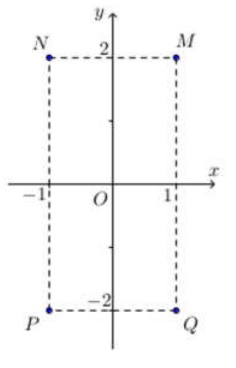
\includegraphics[scale =0.5]{toan04}
\end{wrapfigure}
Hỏi điểm biểu
diễn của $z$ là điểm nào trong các điểm $M, N, P, Q$ ở hình bên ?
\datcot[1]
\bonpa
{\sai {Điểm $P$.}}
{\dung{Điểm $Q$.}}
{\sai {Điểm $M$.}}
{\sai {Điểm $N$.}}
\end{question}


\begin{question} %32
Cho số phức  $z=2+5i$. Tìm số phức  $w=iz+\overline{z}$ .
\datcot
\bonpa
{\sai {$w=7-3i$.}}
{\dung{$w=-3-3i$.}}
{\sai {$w=3+7i$.}}
{\sai {$w=-7-7i$.}}
\end{question}


\begin{question} %33
Kí hiệu $z_1, z_2, z_3$ và $z_4$ là bốn nghiệm phức của phương trình $z^4-z^2-12=0$.\\
Tính tổng $T=|z_1|+|z_2|+|z_3|+|z_4|$. 
\datcot
\bonpa
{\sai {$T=4$.}}
{\sai {$T=2\sqrt3$.}}
{\dung{$4+2\sqrt3$.}}
{\sai {$T=2+2\sqrt3$.}}
\end{question}


\begin{question} %34
Cho các số phức $z$ thỏa mãn$ | z | = 4$. Biết rằng tập hợp các điểm biểu diễn các
số phức  $w=(3+4i)z+i$ là một đường tròn. Tính bán kính $r$ của đường tròn đó.
\datcot
\bonpa
{\sai {$r=4$.}}
{\sai {$r=5$.}}
{\dung{$r=20$.}}
{\sai {$r=22$.}}
\end{question}


\begin{question} %35
Tính thể tích $V$ của khối lập phương  $ABCD. A' B' C' D'$ , biết  $AC=a\sqrt3$.
\datcot
\bonpa
{\dung{$V=a^3$.}}
{\sai {$V=\dfrac{3\sqrt6a^3}{4}$.}}
{\sai {$V=3\sqrt3a^3$.}}
{\sai {$V=\dfrac{1}{3}a^3$.}}
\end{question}


\begin{question} %36
Cho hình chóp tứ giác $S.ABCD$ có đáy $ABCD$ là hình vuông cạnh a, cạnh bên
$SA$ vuông góc với mặt phẳng đáy và  $SA=\sqrt2 a$. Tính thể tích $V$ của khối chóp $S.ABCD$.
\datcot
\bonpa
{\sai {$V=\dfrac{\sqrt2 a^3}{6}$.}}
{\sai {$V=\dfrac{\sqrt2 a^3}{4}$.}}
{\sai {$V=\sqrt2 a^3$.}}
{\dung{$V=\dfrac{\sqrt2 a^3}{3}$.}}
\end{question}

\begin{question} %37
 Cho tứ diện $ABCD$ có các cạnh $AB, AC$ và $AD$ đôi một vuông góc với nhau; $AB = 6a$,
$AC = 7a$ và $AD = 4a$. Gọi $M, N, P$ tương ứng là trung điểm các cạnh $BC, CD, DB$. Tính thể tích
$V$ của tứ diện $AMNP$.
\datcot
\bonpa
{\sai {$V=\dfrac{7}{2}a^3$.}}
{\sai {$V=14a^3$.}}
{\sai {$V=\dfrac{28}{3}a^3$.}}
{\dung{$V=7a^3$.}}
\end{question}

\begin{question}%38
Cho hình chóp tứ giác $S.ABCD$ có đáy là hình vuông cạnh bằng $\sqrt2a $. Tam
giác $SAD$ cân tại $S$ và mặt bên $(SAD)$ vuông góc với mặt phẳng đáy. Biết thể tích khối
chóp $S.ABCD$ bằng $\dfrac{4}{3}a^3$. Tính khoảng cách h từ B đến mặt phẳng (SCD).
\datcot
\bonpa
{\sai {$h=\dfrac{2}{3}a$.}}
{\dung{$h=\dfrac{4}{3}a$.}}
{\sai {$h=\dfrac{8}{3}a$.}}
{\sai {$h=\dfrac{3}{4}a$.}}
\end{question}

\begin{question}%39
Trong không gian, cho tam giác $ABC$ vuông tại $A, AB = a$ và   $AC=\sqrt3 a$. Tính
độ dài đường sinh l của hình nón, nhận được khi quay tam giác $ABC$ xung quanh trục $AB$.
\datcot
\bonpa
{\sai {$l=a$.}}
{\sai {$l=\sqrt2a$.}}
{\sai {$l=\sqrt3a$.}}
{\dung{$l=2a$.}}
\end{question}

\begin{question} %40
Từ một tấm tôn hình chữ nhật kích thước 50cm $\times$ 240cm, người ta làm các
thùng đựng nước hình trụ có chiều cao bằng 50cm, theo hai cách sau (xem hình minh
họa dưới đây) :\\
 Cách 1 : Gò tấm tôn ban đầu thành mặt xung quanh của thùng.
\\ 
 Cách 2 : Cắt tấm tôn ban đầu thành hai tấm bằng nhau, rồi gò mỗi tấm đó thành mặt
xung quanh của một thùng.

\begin{wrapfigure}[10]{r}[-5.5cm]{2cm}
\examvspace*{-.5cm}
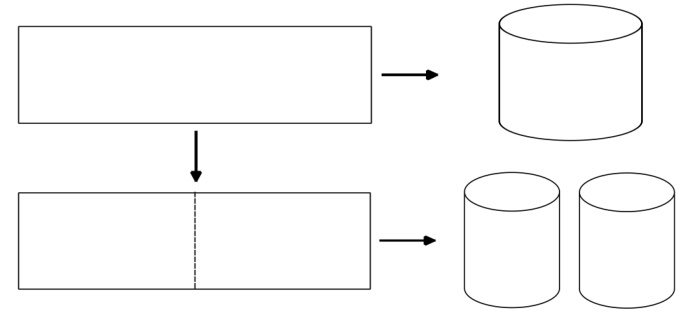
\includegraphics[scale =0.5]{toan05}
\end{wrapfigure}
Kí hiệu $V_1$ là thể tích của thùng gò được theo cách 1 và
$V_2$ là tổng thể tích của hai thùng
gò được theo cách 2. Tính tỉ số $\dfrac{V_1}{V_2}$.
\datcot
\bonpa
{\sai {$\dfrac{V_1}{V_2}=\dfrac{1}{2}$.}}
{\sai {$\dfrac{V_1}{V_2}=1$.}}
{\dung{$\dfrac{V_1}{V_2}=2$.}}
{\sai {$\dfrac{V_1}{V_2}=4$.}}
\end{question}

\begin{question} %41
Trong không gian, cho hình chữ nhật $ABCD$ có $AB = 1$ và $AD = 2.$ Gọi $M, N$
lần lượt là trung điểm của $AD$ và $BC$. Quay hình chữ nhật đó xung quanh trục $MN$, ta
được một hình trụ. Tính diện tích toàn phần $S_{tp} $ của hình trụ đó.
\datcot
\bonpa
{\dung{$S_{tp}=4\pi$.}}
{\sai {$S_{tp}=2\pi$.}}
{\sai {$S_{tp}=6\pi$.}}
{\sai {$S_{tp}=10\pi$.}}
\end{question}

\begin{question} %42
Cho hình chóp $S.ABC$ có đáy $ABC$ là tam giác đều cạnh bằng 1, mặt bên $SAB$ là
tam giác đều và nằm trong mặt phẳng vuông góc với mặt phẳng đáy. Tính thể tích $V$ của
khối cầu ngoại tiếp hình chóp đã cho.
\datcot
\bonpa
{\sai {$V=\dfrac{5\sqrt{15}\pi}{18}$.}}
{\dung{$V=\dfrac{5\sqrt{15}\pi}{54}$.}}
{\sai {$V=\dfrac{4\sqrt{3}\pi}{27}$.}}
{\sai {$V=\dfrac{5\pi}{3}$.}}
\end{question}

\begin{question} %43
Trong không gian với hệ tọa độ $Oxyz$, cho mặt phẳng $(P) : 3x - z + 2 = 0$. Vectơ
nào dưới đây là một vectơ pháp tuyến của (P) ?
\datcot
\bonpa
{\sai {$\overrightarrow{n_4}=(-1;0;-1)$.}}
{\sai {$\overrightarrow{n_1}=(3;-1;2)$.}}
{\sai {$\overrightarrow{n_3}=(3;-1;0)$.}}
{\dung{$\overrightarrow{n_2}=(3;0;-1)$.}}
\end{question}

\begin{question} %44
Trong không gian với hệ tọa độ $Oxyz$, cho mặt cầu
$(S):(x+1)^2+(y-2)^2+(z-1)^2=9.$
Tìm tọa độ tâm $I$ và tính bán kính $R$ của $(S)$.
\datcot[2]
\bonpa
{\dung{$I(-1;2;1)$ và $R=3$.}}
{\sai {$I(1;-2;-1)$ và $R=3$.}}
{\sai {$I(-1;2;1)$ và $R=9$.}}
{\sai {$I(1;-2;-1)$ và $R=9$.}}
\end{question}


\begin{question} %45
Trong không gian với hệ tọa độ $Oxyz$, cho mặt phẳng $(P) $:  
$3x+4y+2z+4=0$
và điểm $A(1; -2; 3).$ Tính khoảng cách $d$ từ $A$ đến ($P$).
\datcot
\bonpa
{\sai {$d=\dfrac{5}{9}$.}}
{\sai {$d=\dfrac{5}{29}$.}}
{\dung{$d=\dfrac{5}{\sqrt{29}}$.}}
{\sai {$d=\dfrac{\sqrt5}{3}$.}}
\end{question}

\begin{question} %46
Trong không gian với hệ tọa độ $Oxyz$, cho đường thẳng $\Delta :
\dfrac{x-10}{5}=\dfrac{y-2}{1}=\dfrac{z+2}{1}.$
Xét mặt phẳng $(P) : 10x + 2y + mz + 11 = 0$, $m$ là tham số thực. Tìm tất cả các giá trị của
$m$ để mặt phẳng $(P)$ vuông góc với đường thẳng $\Delta$.
\datcot
\bonpa
{\sai {$m=-2$.}}
{\dung{$m=2$.}}
{\sai {$m=-52$.}}
{\sai {$m=52$.}}
\end{question}

\begin{question} %47
Trong không gian với hệ tọa độ $Oxyz$, cho hai điểm $A(0; 1; 1)$ và $B(1; 2; 3)$.
Viết phương trình của mặt phẳng $(P)$ đi qua $A$ và vuông góc với đường thẳng $AB$.
\datcot[2]
\bonpa
{\dung{$x + y + 2z - 3 = 0$.}}
{\sai {$x + y + 2z - 6 = 0$.}}
{\sai {$x + 3y + 4z -7 = 0$.}}
{\sai {$ x + 3y + 4z - 26 = 0$.}}
\end{question}

\begin{question} %48
Trong không gian với hệ tọa độ $Oxyz$, cho  mặt
phẳng $(P):  2x+y+2z+2=0$  và mặt cầu ($S$) có tâm $I(2; 1; 1)$. Biết mặt phẳng ($P$) cắt mặt cầu ($S$) theo giao tuyến là
một đường tròn có bán kính bằng 1. Viết phương trình của mặt cầu ($S$).
\datcot
\bonpa
{\sai {$(S)$: $(x+2)^2+(y+1)^2+(z+1)^2=8$.}}
{\sai {$(S)$: $(x+2)^2+(y+1)^2+(z+1)^2=10$.}}
{\sai {$(S)$: $(x-2)^2+(y-1)^2+(z-1)^2=8$.}}
{\dung{$(S)$: $(x-2)^2+(y-1)^2+(z-1)^2=10$.}}
\end{question}

\begin{question} %49
Trong không gian với hệ tọa độ $Oxyz$, cho điểm $A(1; 0; 2)$ và đường thẳng $d$ có
phương trình : $\dfrac{x-1}{1}=\dfrac{y}{1}=\dfrac{z+1}{2}$.
Viết phương trình đường thẳng $\Delta$ đi qua $A$, vuông
góc và cắt $d$.
\datcot[2]
\bonpa
{\sai {$\Delta$: $\dfrac{x-1}{1}=\dfrac{y}{1}=\dfrac{z+2}{1}$.}}
{\dung{$\Delta$: $\dfrac{x-1}{1}=\dfrac{y}{1}=\dfrac{z+2}{-1}$.}}
{\sai {$\Delta$: $\dfrac{x-1}{2}=\dfrac{y}{2}=\dfrac{z-2}{1}$.}}
{\sai {$\Delta$: $\dfrac{x-1}{1}=\dfrac{y}{-3}=\dfrac{z-2}{1}$.}}
\end{question}

\begin{question} %50
Trong không gian với hệ tọa độ $Oxyz$, cho bốn điểm $A(1; -2; 0), B(0; -1; 1)$,
$C(2; 1; -1)$ và $D(3; 1; 4)$. Hỏi có tất cả bao nhiêu mặt phẳng cách đều bốn điểm đó ?
\datcot
\bonpa
{\sai {1 mặt phẳng.}}
{\sai {4 mặt phẳng.}}
{\dung{7 mặt phẳng.}}
{\sai {Có vô số mặt phẳng.}}
\end{question}
 \end{vnmultiplechoice}
\end{document}